% !TEX encoding = UTF-8 Unicode

\documentclass[aspectratio=169]{beamer}
\usepackage[utf8]{inputenc}

%% BIB
\usepackage[style=authoryear,backend=biber,url=false]{biblatex}
\addbibresource{nems.bib}
\addbibresource{yeast.bib}

%% GRAPHICS

\usepackage{graphicx}
\graphicspath{{images/},{figures/}}
\usepackage{tikz}

%% COLORS
\definecolor{UWRed}{HTML}{C5050C}
\definecolor{StrongBlue}{HTML}{3F8FD2}
\definecolor{StrongGreen}{HTML}{36C88E}
\definecolor{StrongRed}{HTML}{9B0000}
\definecolor{MyC}{HTML}{009999}
\definecolor{MyM}{HTML}{990099}
\definecolor{MyY}{HTML}{999900}
\definecolor{MyR}{HTML}{990000}
\definecolor{MyG}{HTML}{009900}
\definecolor{MyB}{HTML}{000099}
\definecolor{ActionRed}{HTML}{990000}

%% SLIDE COLOR SETTINGS
\setbeamercolor{structure}{fg=UWRed}
\setbeamercolor{title page}{fg=white}
\setbeamercolor{title}{fg=white}

%% RM NAV SYMBOLS
\setbeamertemplate{navigation symbols}{}

%% FONTS
\setbeamerfont{title}{size=\huge\bfseries}

%% DRAWING
\usetikzlibrary{fit,calc,arrows,arrows.meta,decorations.pathreplacing,decorations.text,decorations.pathmorphing,backgrounds,fit,positioning,shapes,chains,topaths,matrix}

\def\firstcircle{(90:0.3cm) circle (0.6cm)}
\def\secondcircle{(210:0.3cm) circle (0.6cm)}
\def\thirdcircle{(330:0.3cm) circle (0.6cm)}

\tikzset{%
  link/.style={->,>=angle 45,semithick},
  var/.style={circle,draw,minimum size=1.5em,align=center, inner sep=0pt, anchor=center},
  text block/.style={rectangle, rounded corners, draw=#1, fill=white, thick, text width=5em, align=center},
  thick arrow/.style={
     -{Triangle[angle=120:1pt 1]},
%     -Triangle,
     line width=2em, 
     draw=SoftBlue
  },
  arrow label/.style={
    text=white,
    font=\sf,
    align=center
  },
  set mark/.style={
    insert path={
      node [midway, arrow label, node contents=#1]
    }
  },
  set vertical mark/.style={
    insert path={
      node [midway, arrow label, node contents=#1, rotate=-90]
    }
  },
  colormap/.pic={code={    
    \fill[MyC] \firstcircle;
    \fill[MyM] \secondcircle;
    \fill[MyY] \thirdcircle;
    
    % C+M, C+Y
    \begin{scope}
      \clip \firstcircle;
      \fill[MyB] \secondcircle;
      \fill[MyG] \thirdcircle;
    \end{scope}
    
    % M+Y, K
    \begin{scope}
      \clip \secondcircle;
      \fill[MyR] \thirdcircle;
      \clip \firstcircle;
      \fill[black] \thirdcircle;
    \end{scope}
    
    \draw[thick, white] \firstcircle;
    \draw[thick, white] \secondcircle;
    \draw[thick, white] \thirdcircle;
    
    \node[white] at (90:0.6cm) {\scriptsize\bf 1};
    \node[white] at (210:0.6cm) {\scriptsize\bf 2};
    \node[white] at (330:0.6cm) {\scriptsize\bf 3};
  }},
  onslide/.code args={<#1>#2}{
    \only<#1>{\pgfkeysalso{#2}}
  }
}

%% LOGO on slides
\logo{\begin{tikzpicture}[overlay]
  \node[anchor=north east,inner sep=0] at (0,86mm) {
\includegraphics[height=10mm]{SMPH_color-flush.pdf}};
\end{tikzpicture}}

%% CONTENT BEGINS

\title{Context-Specific Nested Effect Models}
\subtitle{RECOMB 2018}
\author{Yuriy Sverchkov}
\institute{University of Wisconsin--Madison}
\date{April 24, 2018}

\begin{document}

  {
    \usebackgroundtemplate{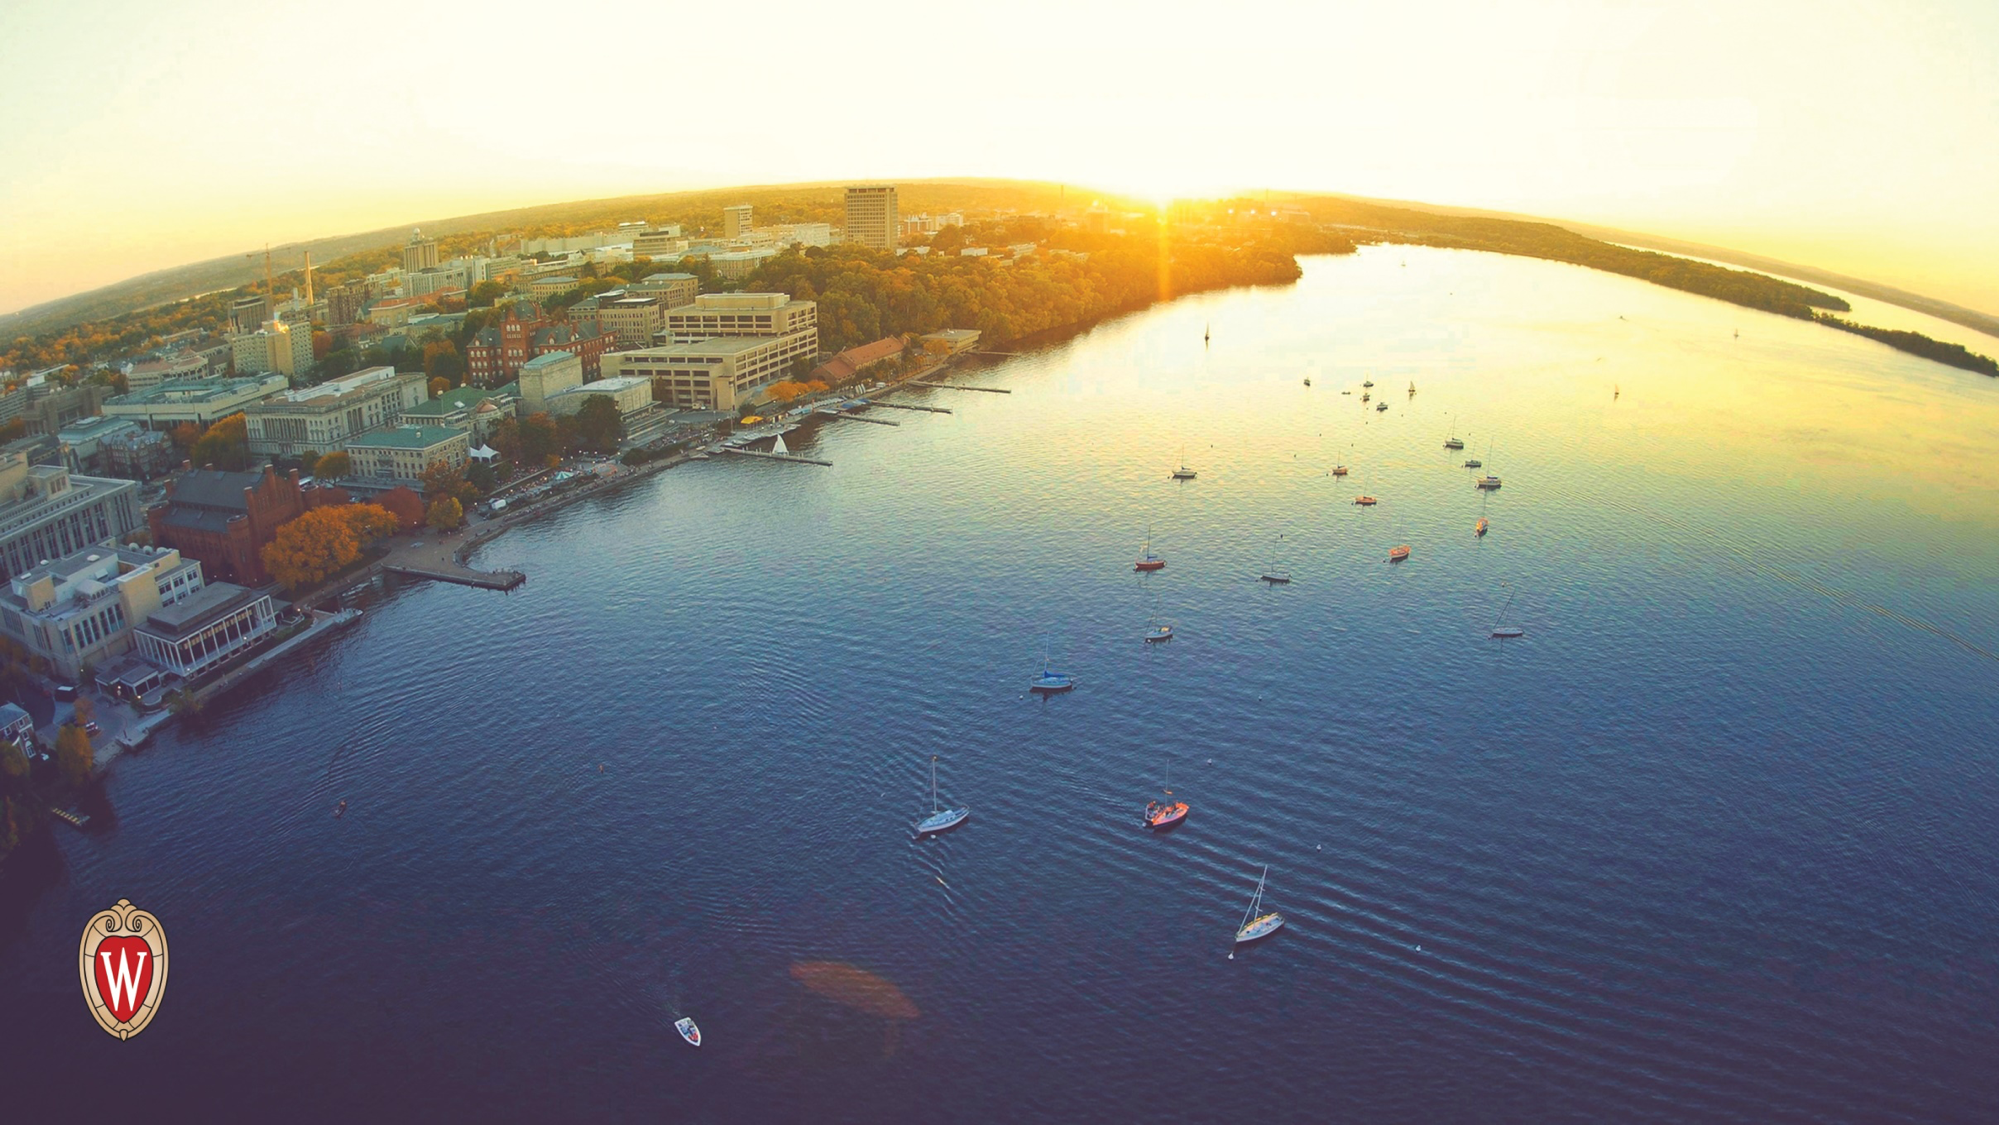
\includegraphics[width=\paperwidth]{UW-lake.png}}
    \begin{frame}[plain]
      \vskip4cm
      \titlepage
    \end{frame}
  }

\begin{frame}{Context-specific biological networks}
\centering
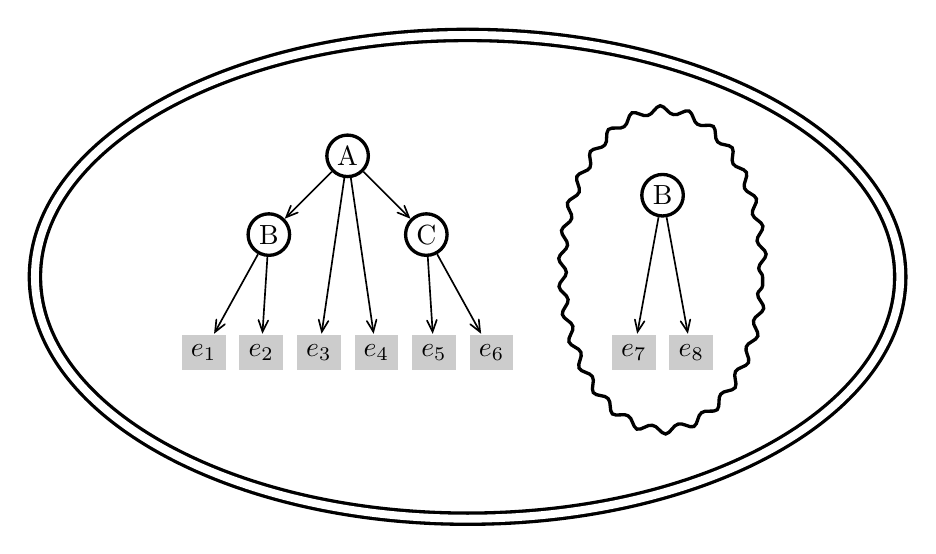
\begin{tikzpicture}[very thick, ampersand replacement=\&]

 \node[var] (a) at (0,5mm) {A};
 \node[var] (b1) at (-1cm,-5mm) {B};
 \node[var] (c) at (1cm,-5mm) {C};
 \node[var] (b2) at (4cm,0) {B};

 \matrix (mr) [matrix of nodes, nodes={fill=black!20}, column sep=0.5em] at (0,-2cm) {
   $e_1$ \& $e_2$ \& $e_3$ \& $e_4$ \& $e_5$ \& $e_6$ \\
 };
 
 \matrix (ml) [matrix of nodes, nodes={fill=black!20}, column sep=0.5em] at (4cm, -2cm) {
   $e_7$ \& $e_8$ \\
 };
 
 \draw[link] (a) to (b1);
 \draw[link] (a) to (c);
 
 \draw[link] (b1) to (mr-1-1);
 \draw[link] (b1) to (mr-1-2);
 \draw[link] (a) to (mr-1-3);
 \draw[link] (a) to (mr-1-4);
 \draw[link] (c) to (mr-1-5);
 \draw[link] (c) to (mr-1-6);
 \draw[link] (b2) to (ml-1-1);
 \draw[link] (b2) to (ml-1-2);
 
 \node[draw, ellipse, fit=(b2) (ml),decoration={snake, amplitude=0.5mm},decorate] (organelle) {};
 \node[draw, ellipse, fit=(a) (b1) (mr) (organelle), double, double distance=1mm] {};

\end{tikzpicture}
\end{frame}
  
%%% FRAMEBREAK %%%

\begin{frame}{Uncovering biological networks}
  \centering
  \begin{tikzpicture}[very thick, ampersand replacement=\&]

    \matrix (es) [matrix of nodes, column sep = 0.5em] at (0,-2cm) {
      \& |[fill=StrongGreen,onslide={<4,5>{fill=StrongRed}}]|$e_1$
      \&  |[fill=StrongGreen,onslide={<4,5>{fill=StrongBlue}}]|$e_2$
      \& |[fill=StrongRed,onslide={<4,5>{fill=StrongBlue}}]|$e_3$
      \& |[fill=StrongRed,onslide={<4>{fill=StrongBlue}}]|$e_4$
      \& |[fill=StrongBlue]|$e_5$
      \& |[fill=StrongGreen,onslide={<4,6>{fill=StrongBlue}}]|$e_6$
      \& |[fill=StrongBlue,onslide={<4,6>{fill=StrongGreen}}]|$e_7$
      \& |[fill=StrongRed,onslide={<4,6>{fill=StrongGreen}}]|$e_8$ \\
    };

    \uncover<3->{
      \node[var] (a) at (0,0) {A};
      \node[var] (b) at (-1cm, -1cm) {B}; 
      \node[var] (c) at (1cm, -1cm) {C};

      \draw[link,onslide=<4>{ActionRed}] (a) to (b);
      \draw[link,onslide=<4>{ActionRed}] (a) to (c);
      \draw[link,{onslide=<4,5>{ActionRed}}] (b) to (es-1-2);
      \draw[link,{onslide=<4,5>{ActionRed}}] (b) to (es-1-3);
      \draw[link,{onslide=<4,5>{ActionRed}}] (b) to (es-1-4);
      \draw[link,onslide=<4>{ActionRed}] (a) to (es-1-5);
      \draw[link,{onslide=<4,6>{ActionRed}}] (c) to (es-1-7);
      \draw[link,{onslide=<4,6>{ActionRed}}] (c) to (es-1-8);
      \draw[link,{onslide=<4,6>{ActionRed}}] (c) to (es-1-9);
    }
    
    \only<4>{
      \draw[very thick, ActionRed] (a.north west) to (a.south east);
      \node[anchor=west, ActionRed] at (a.east) {$\Delta$};
    }
    \only<5>{
      \draw[very thick, ActionRed] (b.north west) to (b.south east);
      \node[anchor=west, ActionRed] at (b.east) {$\Delta$};
    }
    \only<6>{
      \draw[very thick, ActionRed] (c.north west) to (c.south east);
      \node[anchor=west, ActionRed] at (c.east) {$\Delta$};
    }
    
    \node[draw, ellipse, very thick, fit=(a) (b) (c) (es), double, double distance=1mm] (cell) {};

  \matrix (d) [below=5mm of cell, matrix of nodes, nodes={}] {
  \& $e_1$ \& $e_2$ \& $e_3$ \& $e_4$ \& $e_5$ \& $e_6$ \&  $e_7$ \& $e_8$ \\
  WT \& |[fill=StrongGreen]| \&  |[fill=StrongGreen]| \& |[fill=StrongRed]| \& |[fill=StrongRed]| \& |[fill=StrongBlue]| \& |[fill=StrongGreen]| \& |[fill=StrongBlue]| \& |[fill=StrongRed]| \\
  $A\Delta$ \& |[fill=StrongRed]| \&  |[fill=StrongBlue]| \& |[fill=StrongBlue]| \& |[fill=StrongBlue]| \& |[fill=StrongBlue]| \& |[fill=StrongBlue]| \& |[fill=StrongGreen]| \& |[fill=StrongGreen]| \\
  $B\Delta$ \& |[fill=StrongRed]| \&  |[fill=StrongBlue]| \& |[fill=StrongBlue]| \& |[fill=StrongRed]| \& |[fill=StrongBlue]| \& |[fill=StrongGreen]| \& |[fill=StrongBlue]| \& |[fill=StrongRed]| \\
  $C\Delta$ \& |[fill=StrongGreen]| \&  |[fill=StrongGreen]| \& |[fill=StrongRed]| \& |[fill=StrongRed]| \& |[fill=StrongBlue]| \& |[fill=StrongBlue]| \& |[fill=StrongGreen]| \& |[fill=StrongGreen]| \\
 };
  \uncover<1>{ \node[fill=white,fit=(d-2-1) (d-1-9), inner sep=0] {};}
  \uncover<4->{ \node[fill=white,opacity=0.5, fit=(d-2-1) (d-2-9), inner sep=0] {};}
  \node[fill=white,onslide=<4>{opacity=0},onslide=<5-6>{opacity=0.5},fit=(d-3-1) (d-3-9), inner sep=0] {};
  \node[fill=white,onslide=<5>{opacity=0},onslide=<6>{opacity=0.5},fit=(d-4-1) (d-4-9), inner sep=0] {};
  \uncover<-5>{ \node[fill=white,fit=(d-5-1) (d-5-9), inner sep=0] {};}
  
 %   \uncover<7>{
 %     \node[anchor=south, fill=white] at (d.north) {High-dimensional phenotype};
 %   }
  \end{tikzpicture}
\end{frame}

%%% FRAMEBREAK

\begin{frame}{High-dimensional knockout screens}

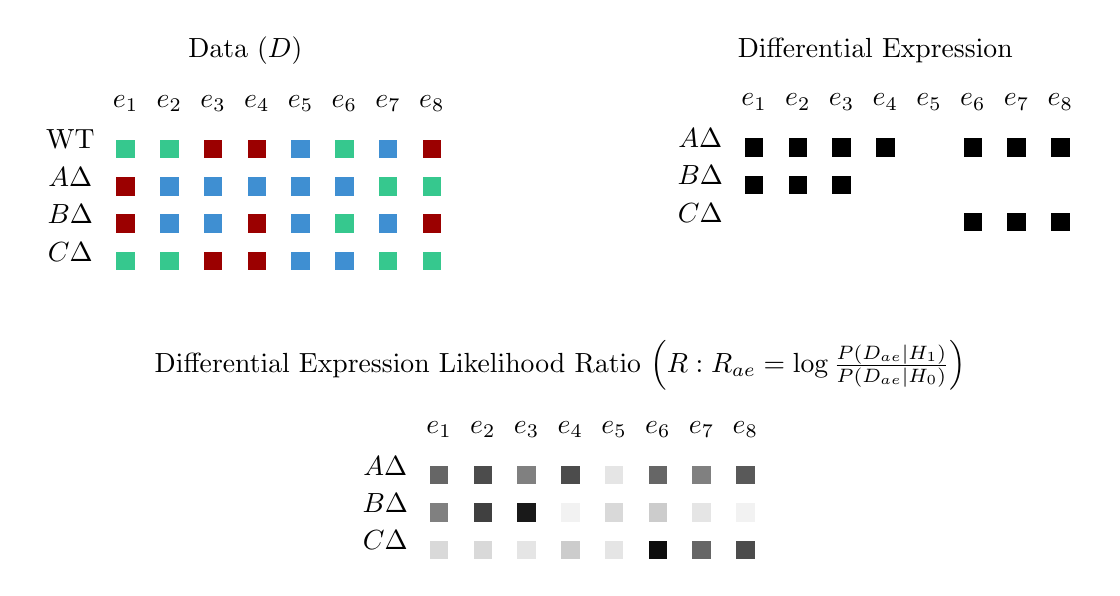
\begin{tikzpicture}[very thick, ampersand replacement=\&]

 \node (data) {Data ($D$)};
 \matrix (dmx) [anchor=north, matrix of nodes] at (data.south) {
  \& $e_1$ \& $e_2$ \& $e_3$ \& $e_4$ \& $e_5$ \& $e_6$ \&  $e_7$ \& $e_8$ \\
  WT \& |[fill=StrongGreen]| \&  |[fill=StrongGreen]| \& |[fill=StrongRed]| \& |[fill=StrongRed]| \& |[fill=StrongBlue]| \& |[fill=StrongGreen]| \& |[fill=StrongBlue]| \& |[fill=StrongRed]| \\
  $A\Delta$ \& |[fill=StrongRed]| \&  |[fill=StrongBlue]| \& |[fill=StrongBlue]| \& |[fill=StrongBlue]| \& |[fill=StrongBlue]| \& |[fill=StrongBlue]| \& |[fill=StrongGreen]| \& |[fill=StrongGreen]| \\
  $B\Delta$ \& |[fill=StrongRed]| \&  |[fill=StrongBlue]| \& |[fill=StrongBlue]| \& |[fill=StrongRed]| \& |[fill=StrongBlue]| \& |[fill=StrongGreen]| \& |[fill=StrongBlue]| \& |[fill=StrongRed]| \\
  $C\Delta$ \& |[fill=StrongGreen]| \&  |[fill=StrongGreen]| \& |[fill=StrongRed]| \& |[fill=StrongRed]| \& |[fill=StrongBlue]| \& |[fill=StrongBlue]| \& |[fill=StrongGreen]| \& |[fill=StrongGreen]| \\
  };
 \uncover<2->{
	\node (de) at (8,0) {Differential Expression};
	\matrix (demx) [anchor=north, matrix of nodes] at (de.south) {
  \& $e_1$ \& $e_2$ \& $e_3$ \& $e_4$ \& $e_5$ \& $e_6$ \&  $e_7$ \& $e_8$ \\
  $A\Delta$ \& |[fill=black]| \&  |[fill=black]| \& |[fill=black]| \& |[fill=black]| \& \& |[fill=black]| \& |[fill=black]| \& |[fill=black]| \\
  $B\Delta$ \& |[fill=black]| \& |[fill=black]| \& |[fill=black]| \& \& \& \& \& \& \& \& \\
  $C\Delta$ \& \& \& \& \& \& |[fill=black]| \& |[fill=black]| \& |[fill=black]| \\
 };
 }
 \uncover<3->{
	\node (lode) at (4,-4) {Differential Expression Likelihood Ratio $\left( R : R_{ae} = \log \frac{ \mathbb P( D_{ae} | H_1 ) }{ \mathbb P( D_{ae} | H_0 ) } \right)$};
	\matrix (lodemx) [anchor=north, matrix of nodes] at (lode.south) {
  \& $e_1$ \& $e_2$ \& $e_3$ \& $e_4$ \& $e_5$ \& $e_6$ \&  $e_7$ \& $e_8$ \\
  $A\Delta$ \& |[fill=black!60]| \&  |[fill=black!70]| \& |[fill=black!50]| \& |[fill=black!70]| \& |[fill=black!10]| \& |[fill=black!60]| \& |[fill=black!50]| \& |[fill=black!65]| \\
  $B\Delta$ \& |[fill=black!50]| \& |[fill=black!75]| \& |[fill=black!90]| \& |[fill=black!5]| \& |[fill=black!15]| \& |[fill=black!20]| \& |[fill=black!10]| \& |[fill=black!5]| \\
  $C\Delta$ \& |[fill=black!15]| \& |[fill=black!15]| \& |[fill=black!10]| \& |[fill=black!20]| \& |[fill=black!10]| \& |[fill=black!95]| \& |[fill=black!60]| \& |[fill=black!70]| \\
 };
 }
\end{tikzpicture}

\end{frame}

%%% FRAMEBREAK %%%

\begin{frame}{Nested effect model (NEM)}

\begin{columns}
\column{0.5\textwidth}

\begin{tikzpicture}[very thick, ampersand replacement=\&]

 {\color{StrongGreen}
  \matrix (es) [anchor=north, matrix of nodes] at (de.south) {
  \& $e_1$ \& $e_2$ \& $e_3$ \& $e_4$ \& $e_5$ \& $e_6$ \&  $e_7$ \& $e_8$ \\
  $A\Delta$ \& |[fill]| \&  |[fill]| \& |[fill]| \& |[fill]| \& \& |[fill]| \& |[fill]| \& |[fill]| \\
  $B\Delta$ \& |[fill]| \& |[fill]| \& |[fill]| \& \& \& \& \& \& \& \& \\
  $C\Delta$ \& \& \& \& \& \& |[fill]| \& |[fill]| \& |[fill]| \\
 };
  \node[anchor=north] at (es.south) {Effect matrix $F$};
 }
 
 \node[var, above=3 of es] (a) {A};
 \node[var, below left=of a] (b) {B}; 
 \node[var, below right=of a] (c) {C};
 
 {\color{StrongBlue}
 \draw[link] (a) to (b);
 \draw[link] (a) to (c);
 }
 {\color{StrongRed}
 \draw[link] (b) to (es-1-2);
 \draw[link] (b) to (es-1-3);
 \draw[link] (b) to (es-1-4);
 \draw[link] (a) to (es-1-5);
 \draw[link] (c) to (es-1-7);
 \draw[link] (c) to (es-1-8);
 \draw[link] (c) to (es-1-9);
 }

\end{tikzpicture}
\pause
\column{0.4\textwidth}

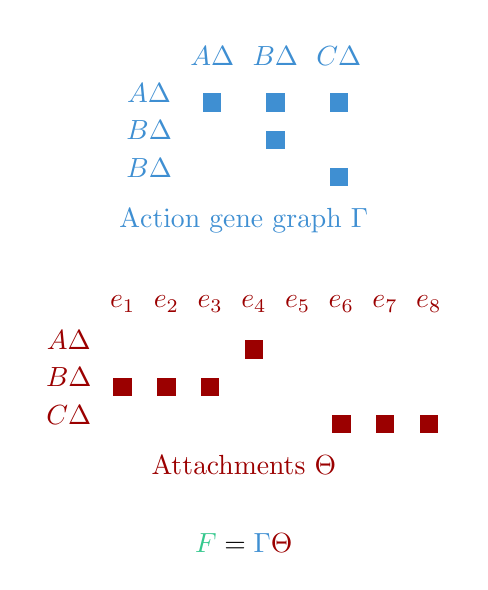
\begin{tikzpicture}[very thick, ampersand replacement=\&]

 {\color{StrongBlue} 
 \matrix (gamma) [matrix of nodes] {
  \& $A\Delta$ \& $B\Delta$ \& $C\Delta$ \\
  $A\Delta$ \& |[fill]| \&  |[fill]| \& |[fill]| \\
  $B\Delta$ \& \& |[fill]| \& \\
  $B\Delta$ \& \& \&  |[fill]| \\
 };
 \node[anchor=north] at (gamma.south) {Action gene graph $\Gamma$};
 }
 
 {\color{StrongRed}
 \matrix (theta) [below=of gamma, matrix of nodes] {
  \& $e_1$ \& $e_2$ \& $e_3$ \& $e_4$ \& $e_5$ \& $e_6$ \&  $e_7$ \& $e_8$ \\
  $A\Delta$ \& \& \& \& |[fill]| \& \& \& \& \\
  $B\Delta$ \& |[fill]| \& |[fill]| \& |[fill]| \& \& \& \& \& \& \& \& \\
  $C\Delta$ \& \& \& \& \& \& |[fill]| \& |[fill]| \& |[fill]| \\
 };
 \node[anchor=north] at (theta.south) {Attachments $\Theta$};
 }
 
 \node (formula) [below=of theta] {${\color{StrongGreen} F} = {\color{StrongBlue} \Gamma} {\color{StrongRed}\Theta}$};

\end{tikzpicture}

\end{columns}

{\tiny \parencite{Markowetz01012005}} %TODO: Add more
\end{frame}

%%% FRAMEBREAK %%%

\begin{frame}{Context-specific nested effect model (CSNEM)}
\centering
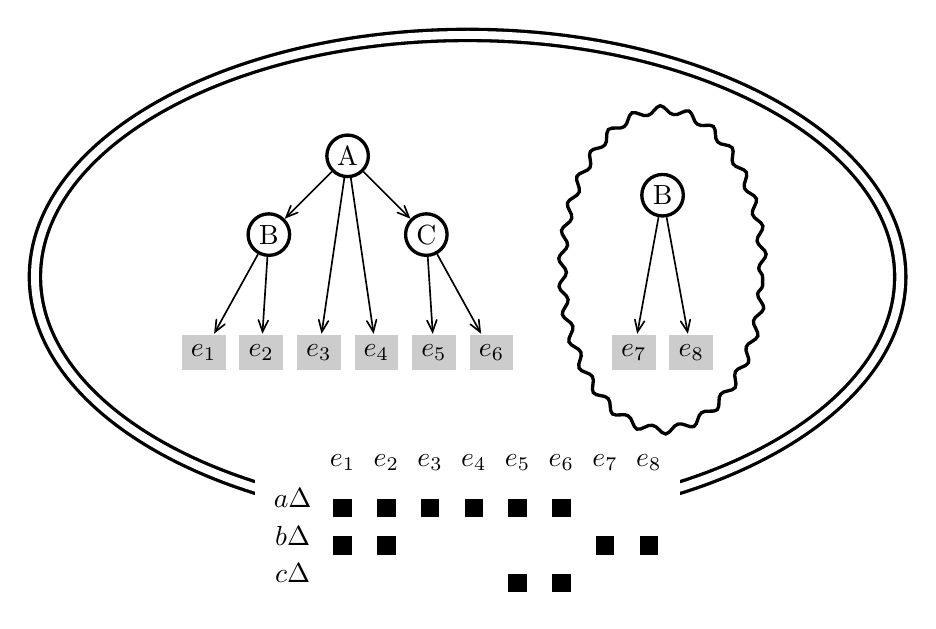
\begin{tikzpicture}[very thick, ampersand replacement=\&]

 \node[var] (a) at (0,5mm) {A};
 \node[var] (b1) at (-1cm,-5mm) {B};
 \node[var] (c) at (1cm,-5mm) {C};
 \node[var] (b2) at (4cm,0) {B};

 \matrix (mr) [matrix of nodes, nodes={fill=black!20}, column sep=0.5em] at (0,-2cm) {
   $e_1$ \& $e_2$ \& $e_3$ \& $e_4$ \& $e_5$ \& $e_6$ \\
 };
 
 \matrix (ml) [matrix of nodes, nodes={fill=black!20}, column sep=0.5em] at (4cm, -2cm) {
   $e_7$ \& $e_8$ \\
 };
 
 \draw[link] (a) to (b1);
 \draw[link] (a) to (c);
 
 \draw[link] (b1) to (mr-1-1);
 \draw[link] (b1) to (mr-1-2);
 \draw[link] (a) to (mr-1-3);
 \draw[link] (a) to (mr-1-4);
 \draw[link] (c) to (mr-1-5);
 \draw[link] (c) to (mr-1-6);
 \draw[link] (b2) to (ml-1-1);
 \draw[link] (b2) to (ml-1-2);
 
 \node[draw, ellipse, fit=(b2) (ml),decoration={snake, amplitude=0.5mm},decorate] (organelle) {};
 \node[draw, ellipse, fit=(a) (b1) (mr) (organelle), double, double distance=1mm] (cell) {};

 \uncover<2->{
 \matrix (mx) [matrix of nodes, fill=white, below=2cm of cell.center] {
  \& $e_1$ \& $e_2$ \& $e_3$ \& $e_4$ \& $e_5$ \& $e_6$ \&  $e_7$ \& $e_8$ \\
  $a\Delta$ \& |[fill=black]| \&  |[fill=black]| \& |[fill=black]| \& |[fill=black]| \& |[fill=black]| \& |[fill=black]| \& \& \\
  $b\Delta$ \& |[fill=black]| \& |[fill=black]| \& \& \& \& \& |[fill=black]| \& |[fill=black]| \\
  $c\Delta$ \& \& \& \& \& |[fill=black]| \& |[fill=black]| \& \& \\
 };
 }


\end{tikzpicture}
\end{frame}

%%% FRAMEBREAK %%% TODO:CONTINUE FROM HERE

%%% FRAMEBREAK %%%

%%% FRAMEBREAK %%%

\begin{frame}{CSNEM as a mixture of NEMs}
\centering
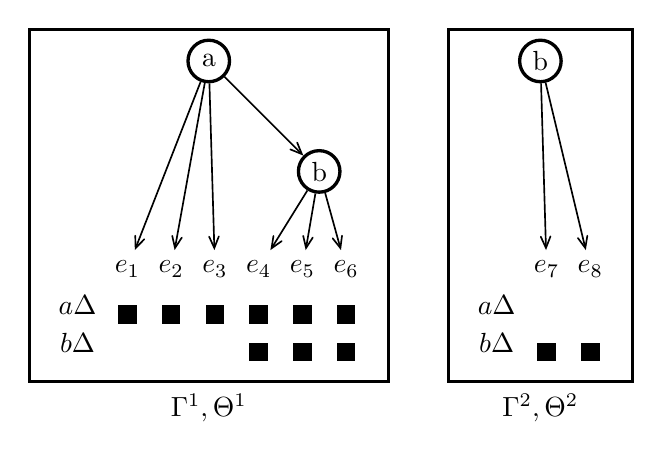
\begin{tikzpicture}[very thick, ampersand replacement=\&]

 \node[var] (a) {a};
 \node[var, below right=1 and 1 of a] (b) {b};
 
  \matrix (mx1) [matrix of nodes, below=2 of a] {
  \& $e_1$ \& $e_2$ \& $e_3$ \& $e_4$ \& $e_5$ \& $e_6$ \\
  $a\Delta$ \& |[fill=black]| \&  |[fill=black]| \& |[fill=black]| \& |[fill=black]| \& |[fill=black]| \& |[fill=black]| \\
  $b\Delta$ \& \& \& \& |[fill=black]| \& |[fill=black]| \& |[fill=black]| \\
 };

  \matrix (mx2) [matrix of nodes, right=of mx1] {
  \& $e_7$ \& $e_8$ \\
  $a\Delta$ \& \& \\
  $b\Delta$ \& |[fill=black]| \& |[fill=black]| \\
 };

 \node[var, above=2 of mx2] (b2) {b};

 \draw[link] (a) to (b);
 \draw[link] (a) to (mx1-1-2);
 \draw[link] (a) to (mx1-1-3);
 \draw[link] (a) to (mx1-1-4);
 \draw[link] (b) to (mx1-1-5);
 \draw[link] (b) to (mx1-1-6);
 \draw[link] (b) to (mx1-1-7);
 \draw[link] (b2) to (mx2-1-2);
 \draw[link] (b2) to (mx2-1-3);

 \node[draw, fit=(a)(mx1)] (nem1) {};
 \node[draw, fit=(b2)(mx2)] (nem2) {};

 \node[anchor=north] at (nem1.south) {$\Gamma^1, \Theta^1$};
 \node[anchor=north] at (nem2.south) {$\Gamma^2, \Theta^2$};

\end{tikzpicture}
\end{frame}

%%% FRAMEBREAK %%%

\begin{frame}{Likelihood formulation}
\[
L_\text{CSNEM}(\Gamma, \Theta) = \prod_{i=1}^k L_\text{NEM}(\Gamma^i, \Theta^i)
\]
\pause
\[
\log L_\text{NEM}(\Gamma^i, \Theta^i) = \sum_{(a,e) \in \mathcal A \times \mathcal E} \log \mathbb P ( D_{ae} | (\Gamma^i \Theta^i)_{ae} ) \pause = \mathsf{tr} ( \Gamma^i \Theta^i R^i ) + c
\]
\pause
\[ \cdots \]
\[
\log L_\text{CSNEM}(\Gamma, \Theta) = \mathsf{tr}( \Gamma \Theta R^* ) + c^*
\]
\end{frame}

%%% FRAMEBREAK %%%

\begin{frame}{Likelihood of a $k$-CSNEM}
\[
L_\text{CSNEM}( \Gamma^1, \ldots, \Gamma^k, \Theta^1, \ldots, \Theta^k )
 = \prod_{i=1}^k L_\text{NEM}( \Gamma^i, \Theta^i ) \]
\pause
\[
\log L_\text{NEM}(\Gamma^i, \Theta^i) = \sum_{(a,e) \in \mathcal A \times \mathcal E} \log \mathbb P ( D_{ae} | (\Gamma^i \Theta^i)_{ae} ) \pause = \mathsf{tr} ( \Gamma^i \Theta^i R^i ) + c
\]
\end{frame}

%%% FRAMEBREAK %%%

\begin{frame}{Likelihood of a $k$-CSNEM}
\begin{multline*}
\log L_\text{CSNEM}( \Gamma^1, \ldots, \Gamma^k, \Theta^1, \ldots, \Theta^k )
 = \\ \text{trace}\left(
 \underbrace{\begin{bmatrix}
	\Gamma^1 & 0 & \cdots & 0 \\
	0 & \Gamma^2 & & \vdots \\
	\vdots & & \ddots & 0 \\
	0 & \cdots & 0 & \Gamma^k
 \end{bmatrix}}_{\text{Block diagonal } \Gamma}
 \underbrace{\begin{bmatrix}
	\Theta^1 & 0 & \cdots & 0 \\
	0 & \Theta^2 & & \vdots \\
	\vdots & & \ddots & 0 \\
	0 & \cdots & 0 & \Theta^k
 \end{bmatrix}}_{\text{``Big'' } (|\mathcal A|k \times |\mathcal E|)\quad \Theta}
 \underbrace{\begin{bmatrix}
	R & R & \cdots & R
 \end{bmatrix}}_{k \text{ copies}} \right) + c
\end{multline*}
\end{frame}

\begin{frame}{Learning approach}
Use MC-EMiNEM \parencite{niederberger2012mc} to solve the modified NEM learning problem.
\[
\log L( \Gamma \Theta ) + \underbrace{\sum_{(a,b) \in \mathcal A \times \mathcal A} \log \mathbb P(\Gamma_{a,b})}_{\text{edge-wise prior}} + \log \mathbb P( \Theta )
\]
\end{frame}

%%% FRAMEBREAK %%%

% Maybe talk about how the simulation works
% > Mixture of random networks (varying density and k)
% > Beta parameter for noise

\begin{frame}{Evaluation on simulated data}
\begin{itemize}[<+->]
 \item \small For each of $n_\mathcal{A} \in \{3,5,10,20\}$ actions, $k_\text{true} \in \{1,\ldots, 5\}$, $\beta \in \{1, 2, 5, 10 \}$
 \item Make a generative $k_\text{true}$-CSNEM model
 \begin{itemize}
  \item Generate $k_\text{true}$ random graphs of $n_\mathcal{A}$ actions.
  \item For each of 1000 effects, with probability 0.7 attach the effect to one of the actions in one of the graphs.
 \end{itemize}
 \item Generate an $n_\mathcal{A} \times 1000$ binary effect matrix $F_\text{true}$ using the CSNEM model
 \item Generate a log-odds matrix $R$ from $F_\text{true}$ by sampling from a $\log \frac{ \mathsf{Beta}(\beta,1) }{ \mathsf{Beta}(1,\beta) }$ distribution where $F_\text{true}$ is 1 and a $\log \frac{ \mathsf{Beta}(1,\beta) }{ \mathsf{Beta}(\beta,1) }$ distribution where $F_\text{true}$ is 0.
 \item For $k_\text{learning} \in \{ 1, \ldots 8 \}$, learn a $k_\text{true}$-CSNEM model from R
 \item Compare the predicted binary effect matrix of $F_\text{learning}$ to the ground truth effect matrix $F_\text{true}$
 \item Compare the graphs learned (by using best-matches of each action's context).
\end{itemize}
\end{frame}

%%% FRAMEBREAK %%%

\begin{frame}{Evaluation on simulated data}
%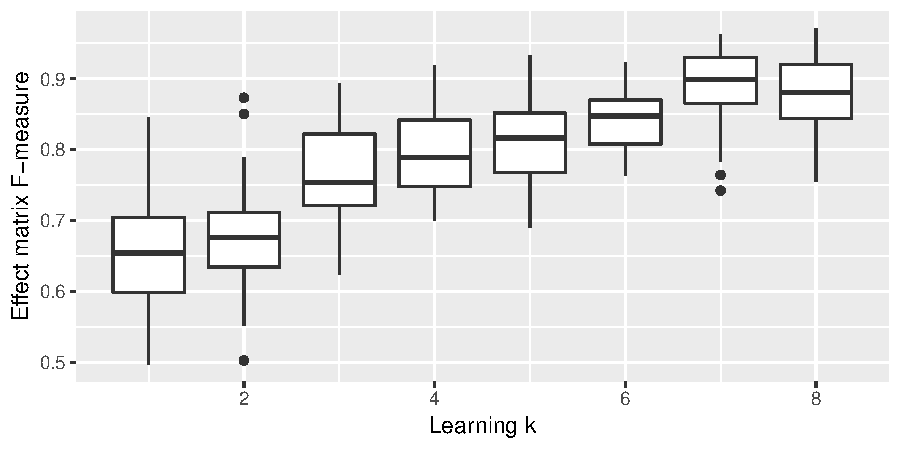
\includegraphics[width=\textwidth]{effect-for-pres}
\end{frame}

%%% FRAMEBREAK %%%

\begin{frame}{Saccharomyces cerevisiae salt stress data}
\begin{itemize}
 \item Wild type strains and 28 single-gene knockout strains
 \item Gene expression measured by microarray
  \begin{itemize}
   \item \normalsize Measurement without salt treatment
   \item \normalsize Measurement 30 minutes after 0.7 M NaCl treatment
  \end{itemize}
 \item Change in response:
\end{itemize}
\[
 \log_2 \left( \frac{\Delta \text{ strain treated}}{\Delta \text{ strain untreated}} \bigg/ \frac{\text{WT strain treated}}{\text{WT strain untreated}} \right)
\]
\vfill
{\tiny \fullcite{berry2008stress} \\ \fullcite{lee2011dynamic} \\}
\end{frame}

%%% FRAMEBREAK %%%

\begin{frame}{}\small  
  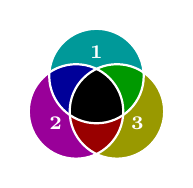
\begin{tikzpicture}
    \path pic {colormap};
  \end{tikzpicture}
\end{frame}

%%% FRAMEBREAK %%%

\begin{frame}{Network learned from the S.\ cerevisiae data}
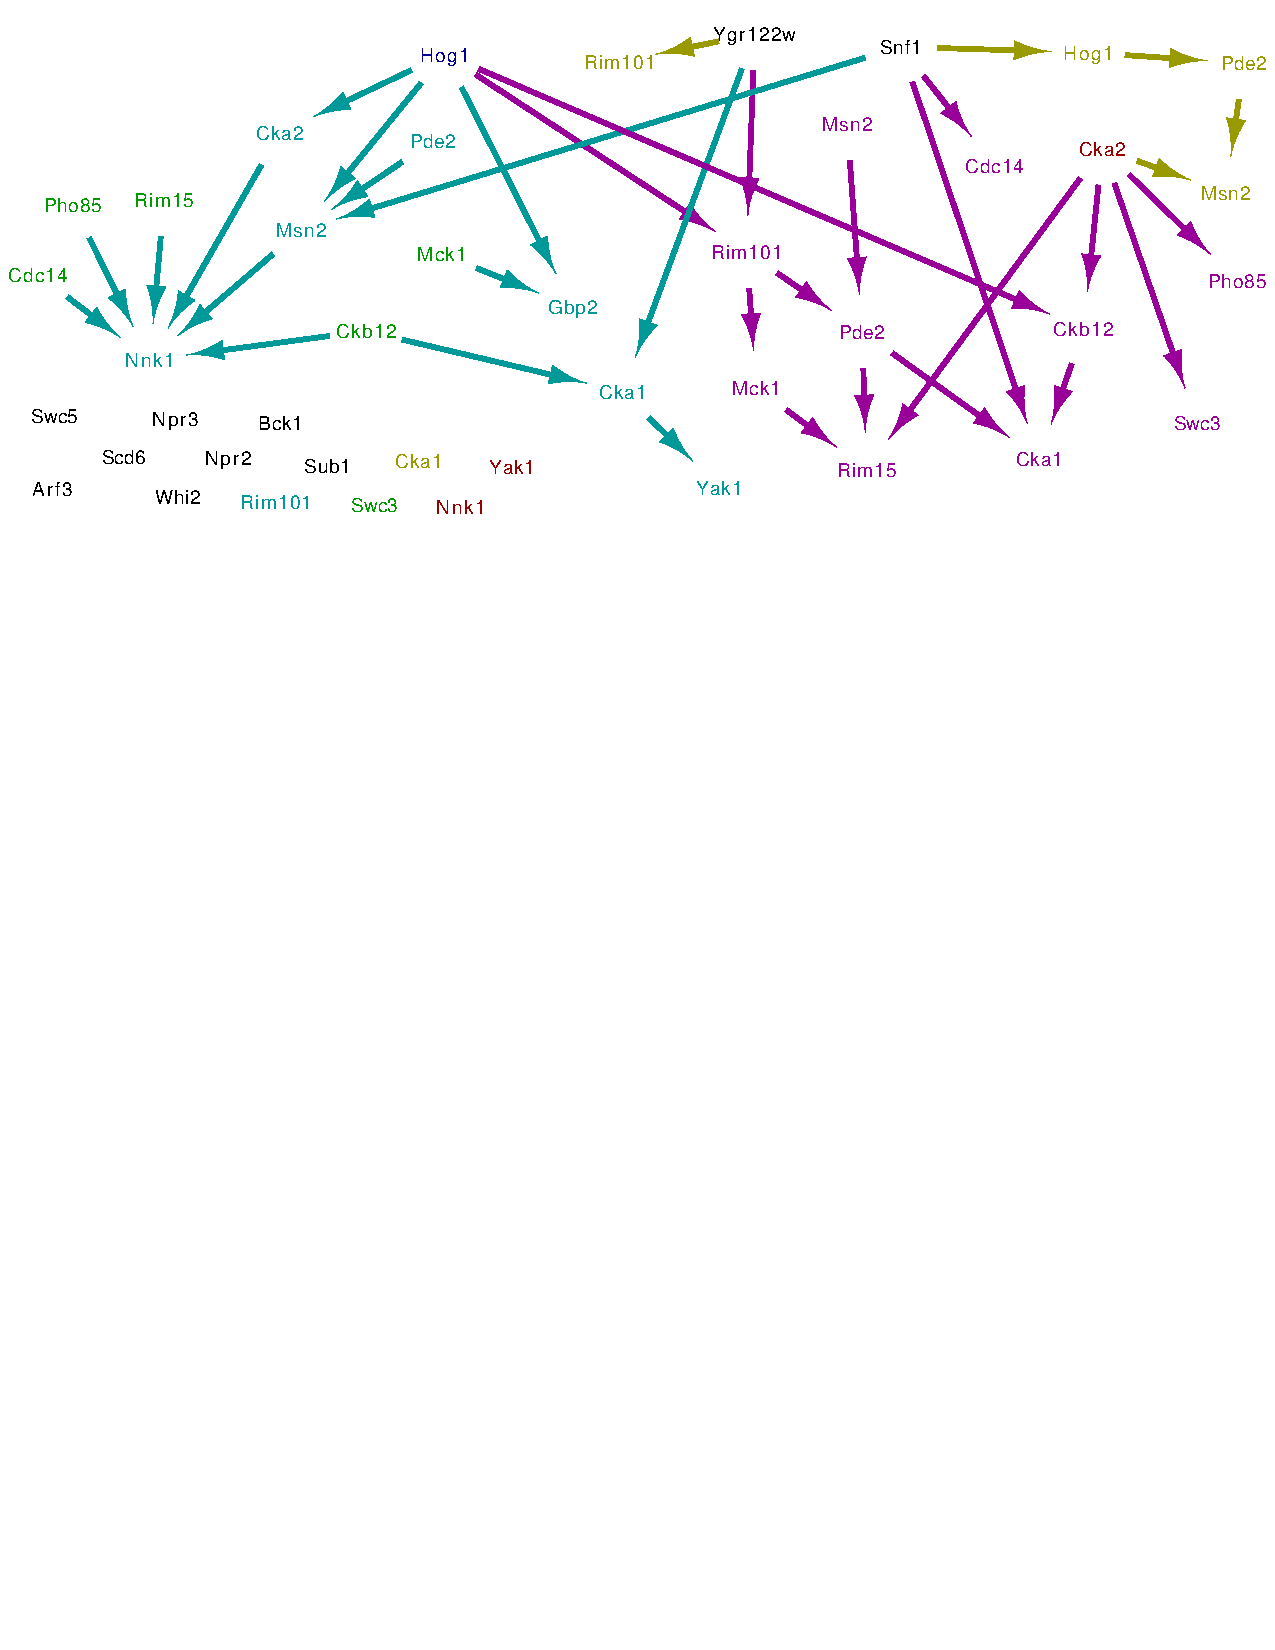
\includegraphics[width=\textwidth]{recomb-2018-short-names.pdf}
\end{frame}

%%% FRAMEBREAK %%%

\begin{frame}{Network learned from the S.\ cerevisiae data}
%\includegraphics[width=\textwidth,trim={0 8.3in 0 0},clip]{hog1-nodes}

\vfill

Hog1 is a master regulator of osmotic stress response
\end{frame}

%%% FRAMEBREAK %%%

\begin{frame}{Network learned from the S.\ cerevisiae data}
%\includegraphics[width=\textwidth,trim={0 8.3in 0 0},clip]{ck-nodes}

\vfill

Hog1 and CK complex subunits (Cka2, Ckb1/2) interact, regulate overlapping sets of genes
\end{frame}

%%% FRAMEBREAK %%%

\begin{frame}{Network learned from the S.\ cerevisiae data}
%\includegraphics[width=\textwidth,trim={0 8in 0 0},clip]{msn2-nodes}

\vfill

Msn2 is known to be regulated by Hog1, Pde2, and Snf1, and Pde2 plays a more significant role in regulating Msn2 during salt stress
\end{frame}

%%% FRAMEBREAK %%%

\begin{frame}{Network learned from the S.\ cerevisiae data}
%\includegraphics[width=\textwidth,trim={0 8in 0 0},clip]{rim101-nodes}

\vfill

YGR122W is required for processing Rim101
\end{frame}

%%% FRAMEBREAK %%%

\begin{frame}{Effect group GO term enrichments}
\centering
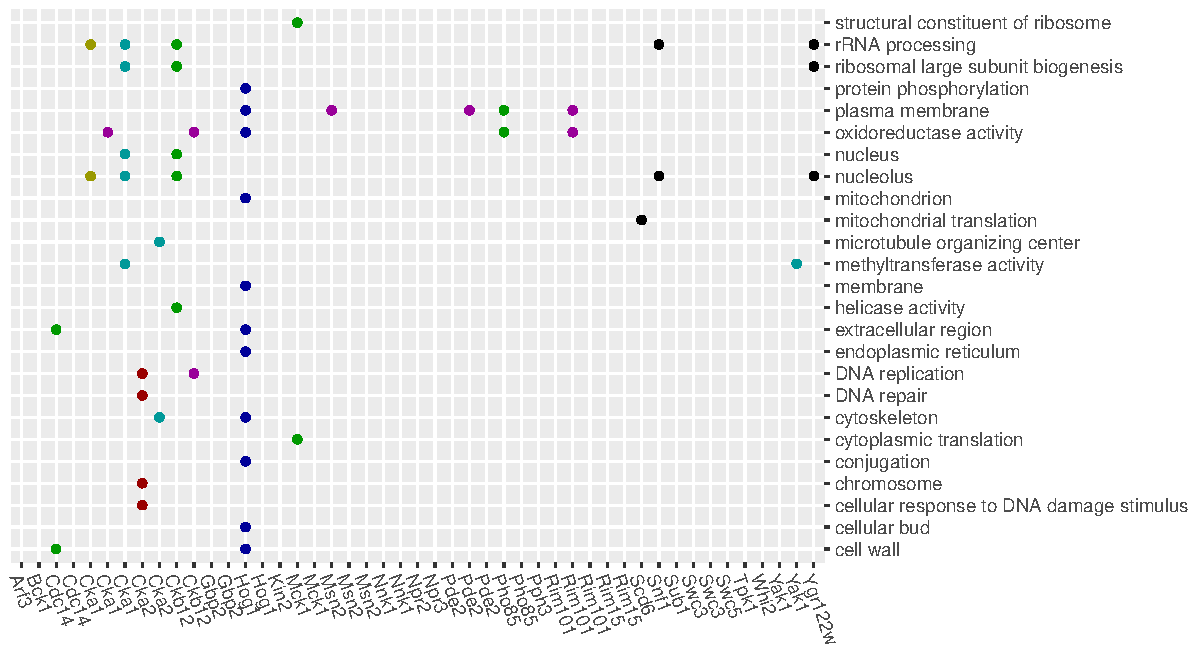
\includegraphics[width=0.8\textwidth]{go-terms-csnem-presentation}
\end{frame}

\begin{frame}{Effect group GO term enrichments}
\centering
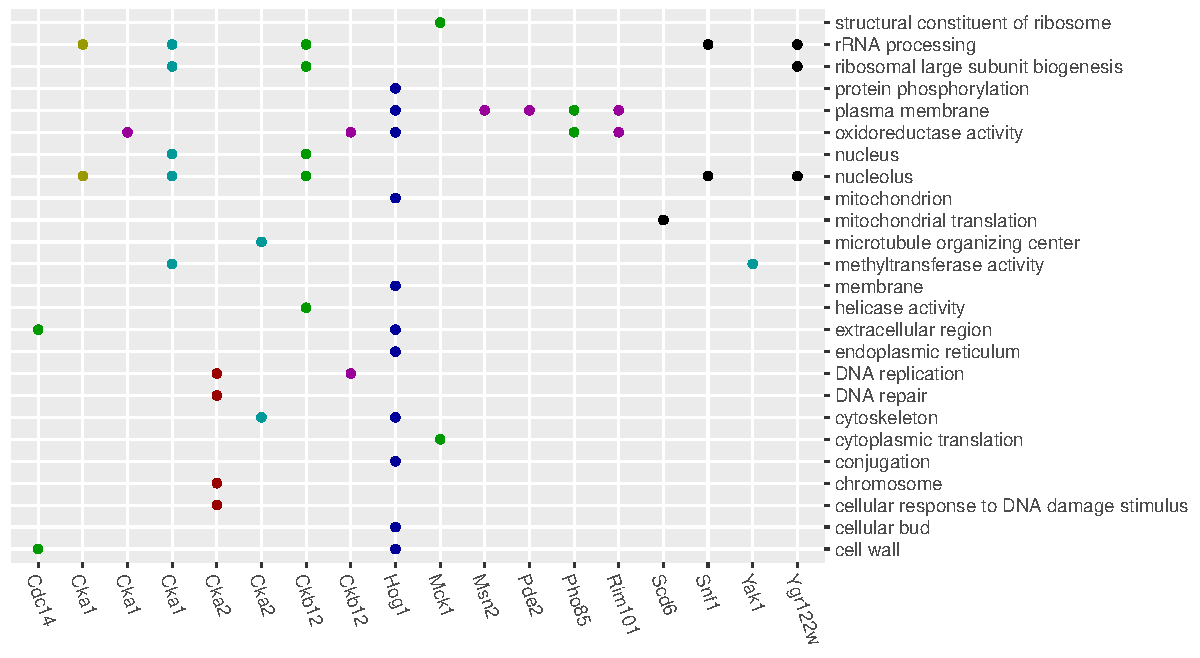
\includegraphics[width=\textwidth]{go-terms-dense-csnem-presentation}
\end{frame}


%%% FRAMEBREAK %%%

\begin{frame}{Context-wise GO term enrichments}
\centering
%\includegraphics{go-term-comparison-contexts-h}
\end{frame}

%%% FRAMEBREAK %%%

\begin{frame}{Conclusions}
 \begin{itemize}
  \item Simulations show that
  \begin{itemize}
   \item context-specificity is recoverable, and
   \item a context-specific model is necessary when the data-generating process is context-specific.
  \end{itemize}
  \item Application to salt-stress data shows
  \begin{itemize}
   \item context-specific effect groups capture meaningful GO categories, and
   \item the learned CSNEM aligns with known biology.
  \end{itemize}
 \end{itemize}
 \pause
 \begin{block}{Acknowledgments}
   Mark Craven, Audrey P. Gash, Elisha Yi-Hsuan Ho %\\
%   CIBM, Grant T15 LM0077359 from the National Library of Medicine, National~Institutes~of~Health
 \end{block}
\end{frame}

%%% FRAMEBREAK %%%

\begin{frame}{Synthesis and identifiability}
\centering
\begin{tikzpicture}[very thick, ampersand replacement=\&]
	\node (n) at (9em, 8em) {\begin{tikzpicture}
		\matrix (n1) [matrix of nodes, row sep=0.5em] {
			Hog1 \& \\
			\& Cka2 \\
			Ckb12 \& \\
		};
		\draw[->] (n1-1-1) -- (n1-2-2);

		\matrix (n2) [right=of n1, matrix of nodes, row sep=0.5em] {
			Hog1 \& \\
			\& Cka2 \\
			Ckb12 \& \\
		};
		\draw[->] (n2-1-1) -- (n2-3-1);
		\draw[->] (n2-2-2) -- (n2-3-1);

		\matrix (n3) [right=of n2, matrix of nodes, row sep=0.5em] {
			Hog1 \& \\
			\& Cka2 \\
			Ckb12 \& \\
		};
		%\draw[->] (n3-1-1) -- (n3-3-1);
		\node [fit=(n1),draw] {};
		\node [fit=(n2),draw] {};
		\node [fit=(n3),draw] {};
	\end{tikzpicture}};
	%\node [anchor=south east] at (n.north west) {(a)};
	
	\node (m) at (0,0) {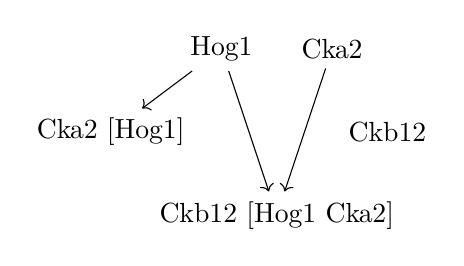
\begin{tikzpicture}
		\node (hog1) at (4em,6em) {Hog1};
		\node (cka2) at (8em,6em) {Cka2};
		\node (cka2-2) at (0,3em) {Cka2 [Hog1]};
		\node (ckb12) at (10em,3em) {Ckb12}; 
		\node (ckb12-2) at (6em,0) {Ckb12 [Hog1 Cka2]};
		\draw[->] (hog1) -- (cka2-2);
		\draw[->] (hog1) -- (ckb12-2);
		\draw[->] (cka2) -- (ckb12-2);
	\end{tikzpicture}};
	%\node at (m.north west) {(b)};
		
	\node (s) at (18em, 0) {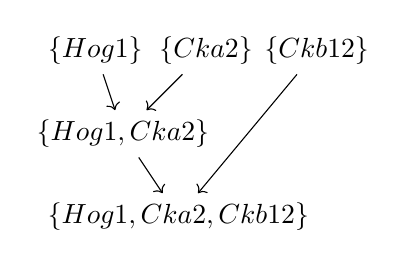
\begin{tikzpicture}
		\node (hog1) at (0,6em) {$\{ \text{Hog1} \}$};
		\node (cka2) at (4em,6em)  {$\{ \text{Cka2} \}$};
		\node (ckb12) at (8em,6em) {$\{ \text{Ckb12} \}$};
		\node (hog1-cka2) at (1em,3em) {$\{ \text{Hog1}, \text{Cka2} \}$};
		\node (all) at (3em,0) {$\{ \text{Hog1}, \text{Cka2}, \text{Ckb12} \}$};
		\draw[->] (hog1) -- (hog1-cka2);
		\draw[->] (cka2) -- (hog1-cka2);
		\draw[->] (hog1-cka2) -- (all);
		\draw[->] (ckb12) -- (all);
	\end{tikzpicture}};
	%\node at (s.north west) {(c)};
	
\end{tikzpicture}
\end{frame}

\end{document}